\section{Generalization}\label{sec_generalization}
A critical component in toolpath generation is how to distribute the beads over the feature radius.
While the framework presented in the previous section takes evenly distributed beads as an example, it allows to apply different beading schemes to configure the bead distribution to cater for specific requirements from the application, 3d printer or material.


% In this section we will generalize the described method into a parametric system, i.e. an algorithmic framework.
% The method we have described above is one for distributing the beads evenly over the total diameter of an outline shape feature.
% Depending on the application, the hardware and the materials used we might need different schemes for determining the bead widths.
% In this section we will generalize the method so that we can apply any distribution of bead widths over a feature radius.
% There are several schemes one can take for determining the distribution of bead widths.
% We will formalize several schemes and describe the set of parameters these schemes require.


\begin{definition}\label{beading_scheme_definition}
The beading scheme is configured by the following set of parameters and functions:
$$
\left\{ \alpha_\text{max}, q(d), t(n), t_0(n), B(n, d) \right\},
$$
where, as introduced in previous section, $\alpha_{\text{max}}$ is the limit bisector angle,
$q(d)$ the quantization operator,
$t(n)$ the transition length,
$t_0(n)$ the transition anchor position
and
$B(n,d)$ is the beading function consisting of $\left( W(n,d), L(n,d) \right)$.
%$W(n, d)$ and $L(n, d)$ give the sequence of bead widths $\left\{ w_i \right\}$ and radial locations $\left\{ l_i \right\}$, respectively.
\end{definition}


The following restrictions hold:
\begin{enumerate}
\item Transitions shouldn't overlap each other: $t_1(n) + t_0(n+1) < \frac{ q^{-1}(n + 1) - q^{-1}(n) }{ \cos \nicefrac12 \alpha_\text{max}}$ for each $n \in \mathbb{N}$ (see \cref{transition_placement})
\item Beadings are symmetric from the center: $W(n, d)_i = W(n, d)_{n-i-1}$ and $L(n, d)_i = d - L(n, d)_{n-i-1}$
%\item $W$ is symmetric: $W(n, d)_i = W(n, d)_{n-i-1}$
%\item $L$ is symmetric in $d$: $L(n, d)_i = d - L(n, d)_{n-i-1}$
\item $W_n$ is positive, monotonic and continuous at each bead index $n$ for constant bead count $c$: $0 \leq \frac{\partial W(c, d)_n}{\partial d} \leq 1$
\end{enumerate}



\begin{figure}
\centering
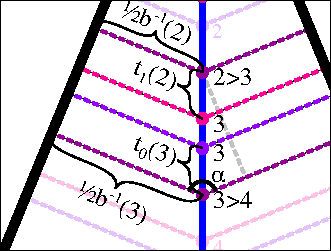
\includegraphics[width=.4\columnwidth]{sources/method/transition_length_limit.pdf}
\caption{
Placement of transition ends (magenta and pink) with respect to the anchor positions of the transitions (purple) on a ST edge (blue) with bisector angle $\alpha \approx \SI{135}{\degree}$.
The distance between the anchor position and the upper end ($t_1$) and the distance between the anchor position and the lower end of the transition ($t_0$) should add up to less than the total distance between the anchor positions, which is limited by $\alpha_\text{max}$.
}
\label{transition_placement}
\end{figure}


Because the peripheral height adjustment was described in terms of a mapping from radial distances to sites rather than adjusting the heights of peripheral nodes,
we can introduce non-linear mappings without refining the surface mesh.
In the simplified geometrical conceptualization of our technique we can introduce different distributions of bead widths from the center outward, by making the contours of the cones curved.
If the UoC mesh is generated with cones which are curving inward toward the top, higher slicing planes would intersect more sparsely than lower ones, which means that the inter-bead distance and thus their width becomes larger when going inward.
In order for the simplified geometrical approach to capture such curved shapes it would have to perform mesh refinement.
However, our approach bypasses the peripheral height adjustment and directly generates the radial distances at the slicing heights, which means our technique generalized effortlessly.




\subsection{Beading schemes}
We introduce several beading schemes which determine the bead count and their widths in various ways.
We can emulate a variety of toolpath generation methods from related literature by defining new beading schemes.
We also introduce new beading schemes which produce toolpaths with less extremal widths compared to techniques from existing literature.

A beading scheme is defined as a set of some particular variables and functions (\cref{beading_scheme_definition}).
Our beading schemes are based on a preferred width $w^* = \SI{0.4}{\milli\meter}$, which is equal to the diameter of the printing nozzle.
Most of the beading schemes we introduce share a common ground:
\begin{align*}
\begin{array}{rlrl}
d_\text{max}^\text{transition} &= \SI{1}{\milli\meter}    &    t_\text{beading} &= w^* \\
d_\text{max}^\text{unmarked} &= w^*    &    t(n) &= w^*  \\ 
d^\text{discretization} &= \SI{0.2}{\milli\meter}    &    t_0(n) &=  t(n) \left( q^{-1}(n) / w^*  - n \right) \\
d_\text{max}^\text{intersection} &= \SI{75}{\percent}     &     \alpha_\text{max} &= \SI{135}{\degree} \\
\end{array} \\
%\end{align*}
%\begin{align*}
L(n,d)_i = 
\begin{cases}
-\frac12 W(n,d)_i + \sum_{j=0}^i W(n,d)_j & \text{ if } i < \frac12 (n -1) \\
d/2 & \text{ if } i =  \frac12 (n -1) \\
d - W(n,d)_{n-1-i} & \text{ otherwise }\\
\end{cases}
\end{align*}

The transition anchor position $t_0$ ensures that the transitions never overlap with the locations $v$ where $2 R(v) = n w^*$ for $n \in \mathbb{N}$.
The transition length $t$ ensures that the center beads don't overlap with the innermost transitioning beads, while keeping the amount of underfill low and keeping the toolpath smooth.
The limit bisector angle $\alpha_\text{max}$ ensures thatwe don't employ transitioning in shallow wedge regions, which would result in a lot of short odd single bead polylines, which would break up the semi-continuous nature of polygonal extrusion paths.
The toolpath locations $L$ ensure 
that the beads don't overlap,
that beads are extruded from the center of where they end up
and that the symmetry restrictions are met.




%\fboxsep=10mm%padding thickness
\begin{figure}%\centering
\setlength{\figwidth}{.2\textwidth}
\setlength{\abovedisplayskip}{0pt}
\setlength{\belowdisplayskip}{0pt}
\captionsetup[subfigure]{justification=justified,singlelinecheck=false}
\fbox{
\begin{subfigure}[b]{\figwidth}\centering
%\frame{
\begin{align*}
\alpha_\text{max} &= \SI{180}{\degree} \\
q^-(d) &= 2 \left\lfloor \frac{d}{ 2w^*} + \frac12 \right\rfloor \\
W(n,d)_i &= w^* \text{ for all } i 
%\\
%L(n,d)_i &= w^* \left(i + \frac12 \right) \text{ for all } i < \frac12 n
\end{align*}
\caption{Uniform scheme}\label{formula_uniform}
\end{subfigure}
}
%
%
\fbox{
\begin{subfigure}[b]{\figwidth}\centering
\begin{align*}
q(d) &=
\begin{cases}
1 & \text{ if } d < w^* \\
2 & \text{ otherwise } \\
\end{cases}
 \\
W(n,d)_i &= 
\begin{cases}
d & \text{ if } n = 1 \\
w^* & \text{ otherwise } \\
\end{cases}
%\\
%L(n,d)_i &= 
%\begin{cases}
%d / 2 & \text{ if } n = 1 \\
%w^* / 2 & \text{ otherwise } \\
%\end{cases}
\end{align*}
\caption{Outer bead}\label{formula_outer_bead}
\end{subfigure}
}
%
%
\fbox{
\begin{subfigure}[b]{\figwidth}\centering
\begin{align*}
\alpha_\text{max} &= \SI{0}{\degree} \\
q(d) &= C \\
W(n,d)_i &= d / n \text{ for all } i 
%\\
%L(n,d)_i &= d / n \left(i + \frac12 \right) \text{ for all } i < \frac12 n
\end{align*}
\caption{Constant bead count}\label{formula_constant_bead_count}
\end{subfigure}
}
%
%
\fbox{
\begin{subfigure}[b]{\figwidth}\centering
\begin{align*}
q(d) &= \left\lfloor \frac{d}{ w^*} + \frac12 \right\rfloor \\
W(n,d)_i &= d / n \text{ for all } i 
%\\
%L(n,d)_i &= d / n (i + \frac12) \text{ for all } i < \frac12 n
\end{align*}
\caption{Evenly distributed}\label{formula_evenly_distributed}
\end{subfigure}
}
%
%
\fbox{
\begin{subfigure}[b]{\figwidth}\centering
\begin{align*}
t(n) &= \frac12 w^* \\
%q^-(d) &= 2 \left\lfloor \frac{d}{ 2w^*} + \frac12 \right\rfloor \\
q(d) &= q^-(d) +
\begin{cases}
-1 & \text{ if } q^-(d) w^* - d > w^* - r_\text{max} \\
1  & \text{ if }  q^-(d) w^* - d < w^* - r_\text{min} \\
0 & \text{ otherwise}
\end{cases}
\\
W(n,d)_i &= 
\begin{cases}
d - (n-1) w^* &\text{ if } i = \frac12 (n-1) \\
w^* &\text{ otherwise }
\end{cases}
%\\
%L(n,d)_i &= 
%\begin{cases}
%d / 2 & \text{ if } i = \frac12 (n-1) \\
%w^* \left(i + \frac12 \right) & \text{ otherwise }
%\end{cases}
\end{align*}
\caption{Centered}\label{formula_centered}
\end{subfigure}
}
%
%
\fbox{
\begin{subfigure}[b]{\figwidth}\centering
\begin{align*}
q(d) &= \left\lfloor \frac{d}{ w^*} + \frac12 \right\rfloor \\
E(n,d) &= d - n w^* \\
W(n,d)_i &= w^* + E(n,d) \frac{M(n,d)_i}{\sum_{j=0}^{n-1} M(n,d)_j} \text{ for all } i \\
%L(n,d)_i &= d / n (i + \frac12) \text{ for all } i < \frac12 n
M(n,d)_i &= \max(0, 1 - \frac{1}{N^2} (i - (n-1)/2)^2 )
\end{align*}
\caption{Inward distributed}\label{formula_inward_distributed}
\end{subfigure}
}
\caption{
Beading schemes.
}
\label{beading_schemes}
\end{figure}


\paragraph{Uniform beading scheme}
We can define a beading scheme which emulates the uniform width offsetting technique by disabling the marking of edges, so that we never employ transitioning.
See \cref{formula_uniform}.


\paragraph{Outer bead}
We can emulate the method by \citeauthor{Moesen2011} by carefully choosing how the beading scheme functions deal with the outermost bead.
Also we turn off the reduction of toolpaths near 3-way intersections $d_\text{max}^\text{intersection} = \SI{0}{\percent}$, so that the polygonal toolpaths emulate the remaining area to be filled by another path planning technique similar to their technique.
We don't need transitioning, so we also set $t(n) = 0 $.
See \cref{formula_outer_bead}.



\paragraph{Constant bead count}
We can emulate the method by \citeauthor{Ding2016a}, by dividing the feature diameter over the widths of a constant number of beads.
Additionally in order to emulate their definition of branches we mark all ST edges and in a separate algorithm we unmark the outer edges connected to the outline shape.
Note that this deviation from the proposed framework violates the robustness against small perturbations in the outline polygon, since the topology of the graph of the ST is not stable against those.
See \cref{formula_constant_bead_count}.




\paragraph{Centered}
We can emulate the method by \citeauthor{Jin2017JMS}, by transcribing how they deviate from the uniform width toolpaths.
We therefore base the beading scheme on the bead count $q^-(d)$ defined by the uniform beading scheme.
\citeauthor{Jin2017JMS} replace two beads from the uniform toolpaths by a single one when the radius between the center and either of those beads falls short of $r_\text{min} = 0.8 w^*$.
Conversely, they place an extra bead when the radius between the center and either of the innermost beads exceeds $r_\text{max} = 1.25 w^*$.\cite{Jin2017JMS}
We emulate the rounded polygonal path rerouting they define by supplying a transition length which results in a discretized version of the rounded polygon segment.
See \cref{formula_centered}.






\paragraph{Evenly distributed}
By taking the advantages of the above two schemes we can define a beading scheme which constitutes a novel toolpathing technique.
We can evenly divide the local feature diameter over the widths of all beads, but choose a local bead count better matching the local feature size.
We determine the local bead count by dividing the diameter by the prefered bead width and rounding to the nearest integer.
This reduces the demands on the system and deviation from mechanical properties caused by beads with extreme deviations from the preferred width.
See \cref{formula_evenly_distributed}.






\paragraph{Inward distributed scheme}
The evenly distributed scheme can be conceptualized as calculating the total discrepancy $E$ between the actual feature diameter $d$ and the total preferred width $n w^*$, dividing the total discrepancy by the number of beads and setting the width of each bead to 
$w^* + E / n$.
However, depending on the application we might want a different distribution of widths.
We therefore supply a beading scheme which supports an arbitrary distribution of the discrepancy.
The distribution is determined by some weighing function $M(n.d)$, which defines the portion of the discrepancy to distribute to each bead.
%\paragraph{Inward distributed}
For example, we can choose an $M$ which distributes the discrepancy over the innermost beads, and distribute most of it to the inner beads.
See \cref{distributed_comparison}.
That way we limit the region of impact of the distributed scheme to a central region and have the nominal bead width $w^*$ in regions farther away.
This limits the impact of transitioning regions so that transitions keep the toolpaths smooth farther away from the central regions. % and it forces most of the beads to have exactly the prefered width.
%Moreover, the bead widths equal the nominal bead width for large regions meaning that mechanical properties derived for prints using the uniform scheme will still hold approximately.
See \cref{formula_inward_distributed}.






\begin{figure}
\centering
\setlength{\figwidth}{.4\columnwidth}
\setlength{\figheight}{.25\columnwidth}
\begin{subfigure}{\figwidth}\centering
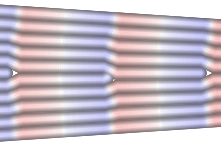
\includegraphics[height=\figheight]{sources/validation/wedge_Distributed_pretty_evenly.png}
\caption{Evenly distributed}
\end{subfigure}
\begin{subfigure}{\figwidth}\centering
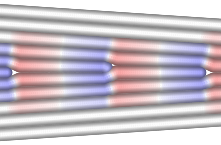
\includegraphics[height=\figheight]{sources/validation/wedge_Distributed_pretty_inward.png}
\caption{Inward distributed}
\end{subfigure}
\begin{subfigure}{.1\columnwidth}\centering
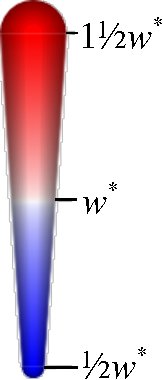
\includegraphics[height=\figheight]{sources/validation/widths_legend_small.pdf}
\end{subfigure}
\caption{
Closeup of toolpaths generated with the distributed beading schemes for a large wedge shape.
Colors represent bead widths.
}
\label{distributed_comparison}
\end{figure}








\paragraph{Widening}
Complementary to any of these schemes we can enforce a minimum feature size at no extra cost in our framework.
Regions where the model is narrower than the nozzle size can be printed with a bead width larger than the model thickness.
We can simply override
\begin{align*}
W'(n,d)_1 &=
\begin{cases}
\max \left( w_\text{nozzle}  ,  W(n,d)_1 \right) & \text{ if } n = 1 \\
W(n,d)_1 & \text{ otherwise}
\end{cases}
\end{align*}




















